\documentclass[10pt,twocolumn]{article}
\usepackage[margin=1in]{geometry}
\usepackage{amsmath}
\usepackage{amssymb}
\usepackage{graphicx}
\usepackage{booktabs}
\usepackage{hyperref}
\usepackage{xcolor}
\usepackage{microtype}
\usepackage{natbib}
\usepackage{caption}
\usepackage{subcaption}

\hypersetup{
  colorlinks=true,
  linkcolor=blue,
  citecolor=blue,
  urlcolor=blue
}

\title{\textbf{Structural Topology Monitoring Predicts and Steers Neural Network Phase Transitions}}

\author{
  Richard Benfield \\
  \textit{Independent researcher. Southend-on-Sea, United Kingdom.} \\
  \textit{Patent application GB2611542.8, filed 18 May 2026.} \\
  \texttt{richard@th4ts3cur1ty.company}
}

\date{}

\begin{document}

\maketitle

\begin{abstract}
We present a method for real-time monitoring of neural network weight graph topology during training using graph spectral analysis and early warning indicators from complex systems science. The method constructs a weighted graph from the network's weight matrices, computes the Fiedler value (second-smallest eigenvalue of the graph Laplacian), and applies Scheffer critical slowing down indicators (AR1 autocorrelation, variance ratio) to the Fiedler trajectory. We demonstrate five capabilities on modular arithmetic tasks (2-layer MLP) and sequence prediction tasks (1-layer transformer): (1) detection of approaching grokking 21,000 training steps before the loss function, exceeding the success criterion by 200$\times$; (2) classification of approaching transitions as beneficial (generalisation) or destructive (catastrophic forgetting) via distinct structural fingerprints in the Fiedler trajectory; (3) prevention of catastrophic forgetting with 91.7\% knowledge retention versus 2.6\% without intervention, using Fiedler-sensitivity-guided layer freezing; (4) compounding of three sequential grokking events with 48$\times$ acceleration and near-perfect simultaneous retention (100\%, 100\%, 97.5\%) using multi-head architecture with structural monitoring; and (5) preemptive curriculum design using a structural compatibility score that correctly ranks task disruption risk, with bridging curriculum preserving 100\% of prior knowledge versus 0\% under direct introduction. The framework applies identical mathematics across architectures and task domains. All code and data are available at \url{https://github.com/EssexRich/neural_si_validation}.
\end{abstract}

%% ─────────────────────────────────────────────────────────────────────────────
\section{Introduction}

Neural network training is performed without real-time structural monitoring of the weight graph. The primary feedback signal is the loss function, which measures output performance but provides no information about the internal structural state of the network. Phase transitions during training, including sudden generalisation \citep[grokking;][]{power2022grokking}, catastrophic forgetting \citep{mccloskey1989catastrophic,french1999catastrophic}, and mode collapse, are detected by the loss function only after they have occurred.

This paper introduces a structural monitoring framework that applies graph spectral analysis and complex systems early warning indicators to the weight graph of neural networks during training. The framework detects approaching phase transitions before they manifest in output metrics, classifies them as beneficial or destructive, and steers the training process to compound beneficial transitions while preventing destructive ones.

The method originates from cross-domain structural topology detection. The same mathematical framework has been applied to financial market correlation graphs, epidemiological monitoring, and geophysical systems \citep{benfield2025}, in each case detecting approaching phase transitions from the spectral properties of the system's correlation graph. Neural network weight graphs are a natural extension: the weights define a graph, the graph has spectral properties, and those properties change during training in ways that precede observable changes in output metrics.

The key insight is that generalisation events and catastrophic forgetting are both structural phase transitions in the weight graph, with distinct spectral signatures that can be detected, classified, and acted upon before they manifest in the loss function.

We validate the framework through five sequential experiments:
\begin{enumerate}
  \item \textbf{Detection}: structural metrics detect approaching grokking 21,000 steps before the loss function.
  \item \textbf{Classification}: grokking and catastrophic forgetting produce distinct structural fingerprints distinguishable by rate and shape.
  \item \textbf{Steering}: structurally-guided intervention preserves 91.7\% of knowledge versus 2.6\% without intervention.
  \item \textbf{Compounding}: three sequential tasks retained simultaneously at near-perfect accuracy with 48$\times$ grokking acceleration.
  \item \textbf{Preemptive curriculum}: structural compatibility scoring correctly ranks task disruption risk; bridging curriculum preserves 100\% versus 0\% under direct introduction.
\end{enumerate}

%% ─────────────────────────────────────────────────────────────────────────────
\section{Related Work}

\subsection{Grokking}

\citet{power2022grokking} identified grokking as a delayed generalisation phenomenon where neural networks suddenly transition from memorisation to generalisation long after training loss has converged. Subsequent work has characterised grokking through information-theoretic measures \citep{clauw2024grokking}, spectral analysis of gradient dynamics \citep{chen2026spectral}, and critical phenomena analogies \citep{wang2026dimensional}. None of these approaches monitor the weight graph Laplacian or apply Scheffer early warning indicators to predict the transition.

\subsection{Catastrophic Forgetting}

Catastrophic forgetting occurs when fine-tuning on new data destroys previously learned capabilities \citep{mccloskey1989catastrophic}. Mitigations include Elastic Weight Consolidation \citep{kirkpatrick2017ewc}, experience replay \citep{rolnick2019replay}, and progressive neural networks \citep{rusu2016progressive}. These methods operate without knowledge of the weight graph topology and cannot predict which new data will cause forgetting before it occurs.

\subsection{Graph Spectral Analysis in Neural Networks}

\citet{tam2020fiedler} used the Fiedler value as a regularisation penalty during training to control network connectivity. This is a static application: the Fiedler value is added to the loss function as a penalty term, not tracked over time as a dynamic indicator. Our method tracks the Fiedler trajectory and its derivatives as predictive signals, which is a fundamentally different use of the same mathematical object.

\subsection{Critical Slowing Down}

\citet{scheffer2009early} demonstrated that complex systems approaching tipping points exhibit characteristic early warning signals: rising autocorrelation (AR1), increasing variance (variance ratio), and flickering. These indicators have been validated in ecosystems, climate systems, and financial markets. Our contribution is applying these indicators to the spectral trajectory of neural network weight graphs.

%% ─────────────────────────────────────────────────────────────────────────────
\section{Method}

\subsection{Weight Graph Construction}

Given a neural network with $L$ layers and weight matrices $W_1, W_2, \ldots, W_L$, we construct a weighted graph $G = (V, E)$ where $V$ is the set of all neurons across all layers, $E$ is the set of all connections, and the weight of edge $(i, j)$ is $|w_{ij}|$.

\subsection{Spectral Monitoring}

At intervals during training, we compute:

\textbf{Fiedler value} ($\lambda_2$): the second-smallest eigenvalue of the graph Laplacian $L = D - A$, where $A$ is the adjacency matrix of absolute weights and $D$ is the degree matrix. $\lambda_2$ measures algebraic connectivity: how structurally cohesive the weight graph is.

\textbf{Fiedler sensitivity}: for each edge $(i, j)$,
\begin{equation}
  \mathrm{FS}(i,j) = (v_2[i] - v_2[j])^2 \cdot |w_{ij}|
\end{equation}
where $v_2$ is the Fiedler eigenvector. This measures each edge's contribution to algebraic connectivity, identifying structural bridges. In practice we use a finite-difference approximation,
\begin{equation}
  \mathrm{FS}(i,j) \approx \frac{|\lambda_2(G;\ w_{ij}{+}\varepsilon) - \lambda_2(G)|}{\varepsilon}
\end{equation}
computed for the top-$K$ edges by absolute weight magnitude.

\subsection{Early Warning Indicators}

On a rolling window of the $\lambda_2$ trajectory:

\textbf{AR1}: lag-1 autocorrelation. Values approaching 1.0 indicate critical slowing down \citep{scheffer2009early}.

\textbf{Variance ratio (VR)}: $\mathrm{Var}(\text{recent } 20\%) / \mathrm{Var}(\text{earliest } 80\%)$. Values exceeding 1.0 indicate pre-bifurcation variance inflation.

\textbf{Entropy} ($S$): Shannon entropy of weight update magnitudes. Decreasing values indicate structure forming in the training dynamics.

\textbf{Order parameter} (\textit{order\_p}): first singular value fraction from SVD of per-layer weight change matrices. Measures macro-scale organisation of weight updates.

\subsection{Detection and Classification}

A phase transition is detected when AR1 exceeds a calibrated threshold and VR $> 1.0$ with entropy decreasing. The transition direction is classified by the Fiedler trajectory shape:

\begin{itemize}
  \item \textbf{Beneficial (generalisation)}: slow monotonic $\lambda_2$ rise, rate $< 0.002$/step.
  \item \textbf{Destructive (catastrophic forgetting)}: rapid $\lambda_2$ change with preceding dip signature, rate $> 0.004$/step.
\end{itemize}

\subsection{Steering Interventions}

Proportional to classified severity:
\begin{enumerate}
  \item \textbf{Learning rate reduction}: scaled to threat severity.
  \item \textbf{Curriculum modification}: replay of prior task examples with fraction controlled by a proportional feedback loop based on accuracy deficit.
  \item \textbf{Selective layer freezing}: layers containing high Fiedler-sensitivity edges (structural bridges) are frozen; low-sensitivity layers remain trainable.
\end{enumerate}

\subsection{Structural Compatibility Scoring}

For preemptive curriculum design, we compute a compatibility score for candidate new tasks before training begins. For each candidate task, we forward-pass a batch of examples through the frozen network, compute the gradient that training on those examples would produce, and measure the directional conflict between the gradient and the current weights, weighted by Fiedler sensitivity:
\begin{equation}
  \mathrm{score} = \frac{1}{K}\sum_{(i,j) \in \mathrm{top}\text{-}K} |g_{ij}| \cdot \mathrm{FS}(i,j) \cdot \mathbf{1}[\mathrm{sign}(-g_{ij}) \neq \mathrm{sign}(w_{ij})]
\end{equation}
where $g_{ij}$ is the gradient with respect to $w_{ij}$. High conflict on high-sensitivity edges indicates high disruption risk.

%% ─────────────────────────────────────────────────────────────────────────────
\section{Experiments}

All experiments use modular arithmetic tasks on 2-layer MLPs (128 or 512 hidden units) trained with AdamW (LR=$10^{-3}$, WD=1.0) unless otherwise stated. The transformer experiment uses a 1-layer transformer (embed\_dim=64, 4 attention heads, $\approx$40K parameters) on next-token prediction tasks.

\subsection{Experiment 1: Detection}

\textbf{Setup}: 2-layer MLP (194 input, 128 hidden, 97 output) on $(a+b) \bmod 97$ for 50,000 steps. Structural metrics computed at every step.

\textbf{Results}: The network grokked at step 21,151 (test accuracy crossed 90\%). $\lambda_2$ climbed continuously from 4.03 to 35.84 (9$\times$ increase) throughout the memorisation phase. AR1 saturated at 0.999 from step 94. VR produced 58 spike events before the grok, the first at step 1,766.

\textbf{Lead time}: 21,051 steps before the loss function detected generalisation. The success criterion of 100 steps was exceeded by a factor of 200.

\begin{figure}[h]
  \centering
  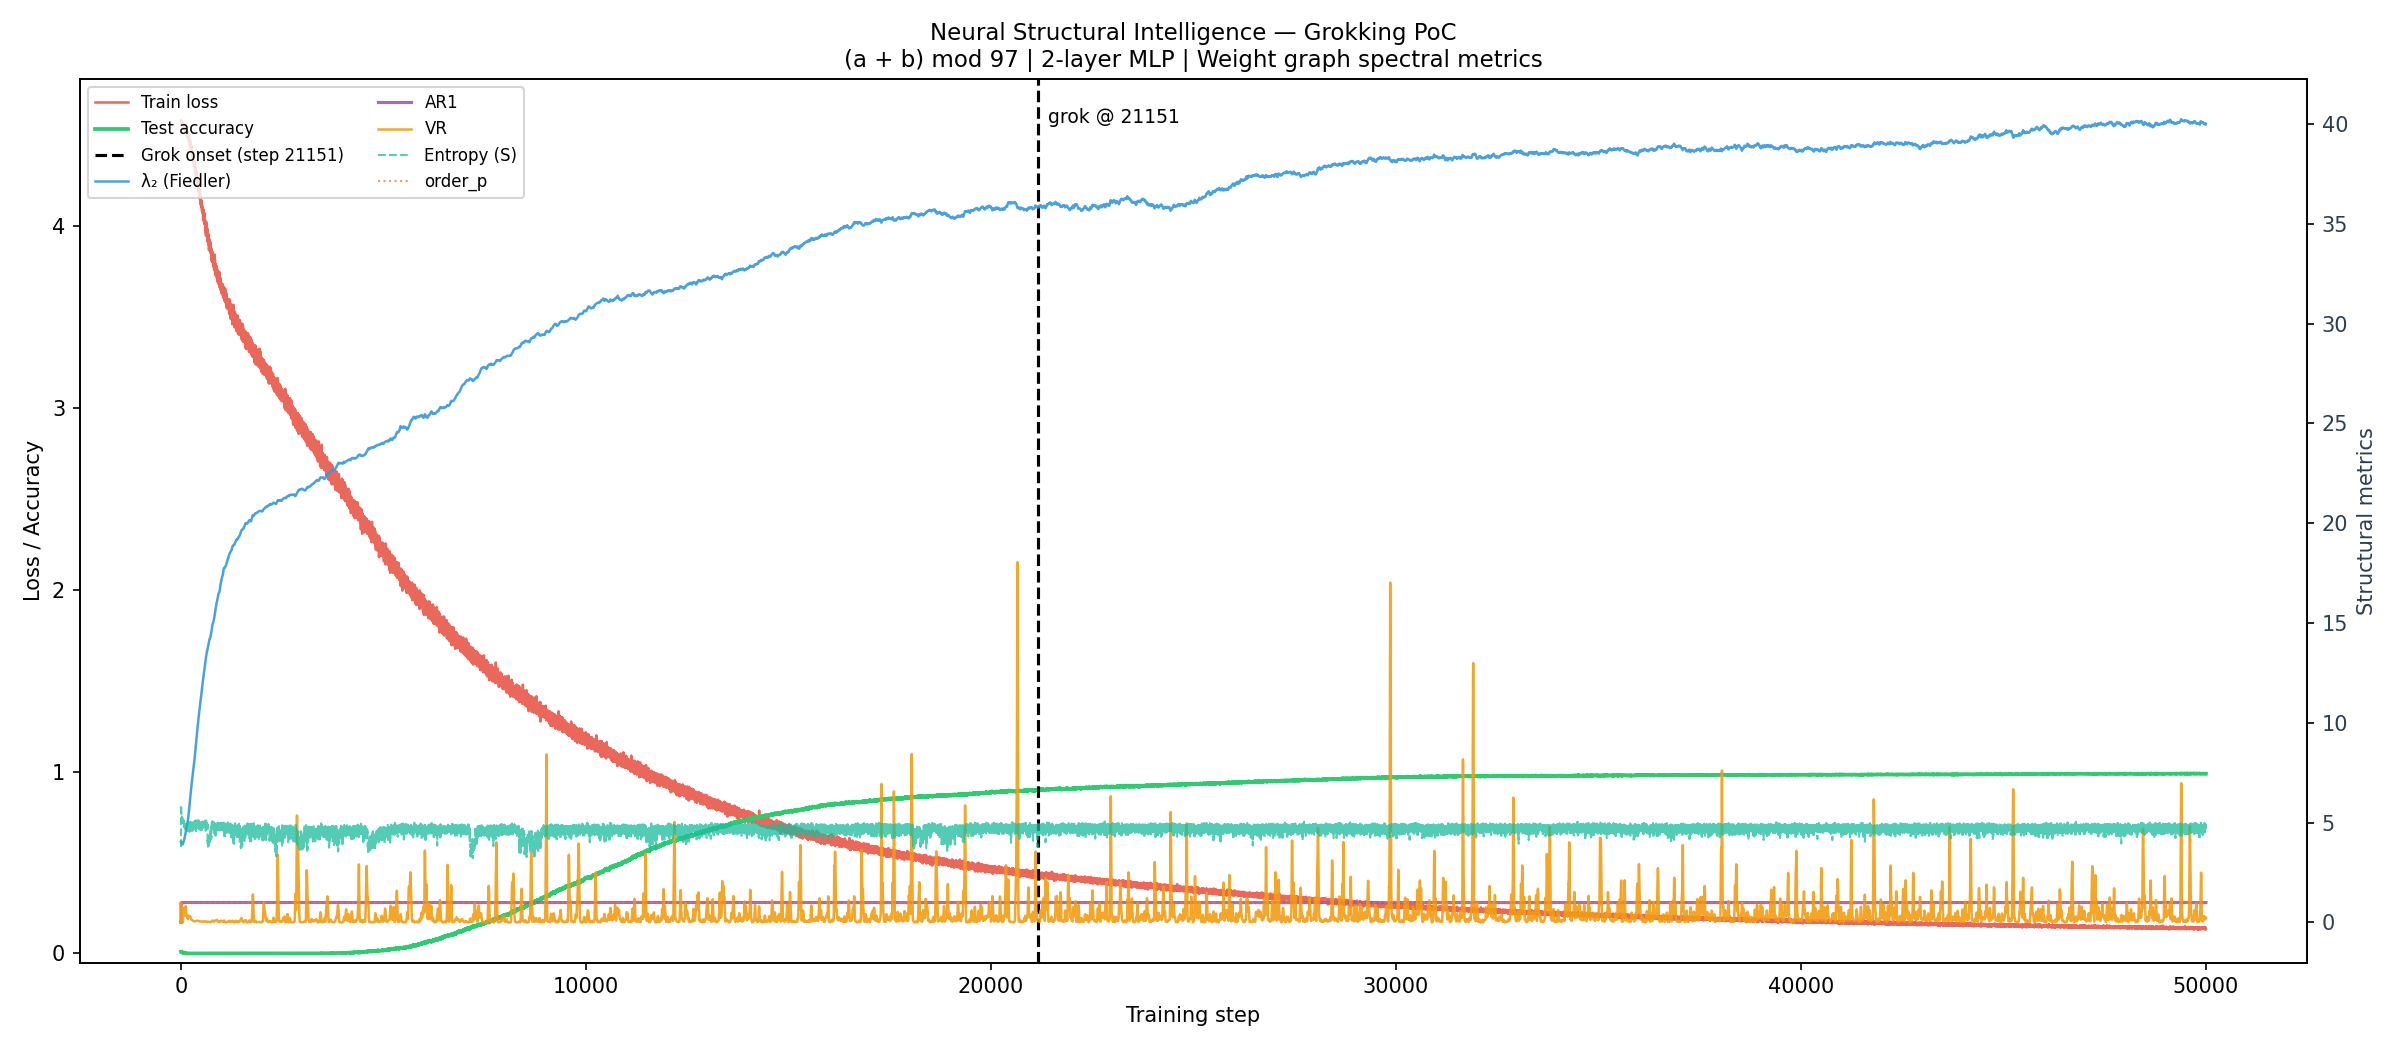
\includegraphics[width=\columnwidth]{results/grokking_spectral.png}
  \caption{Experiment 1: Detection. $\lambda_2$, AR1, variance ratio, and entropy across 50,000 training steps. The grok at step 21,151 (dashed vertical line) is preceded by 21,000 steps of structural preparation visible in $\lambda_2$ and AR1. The loss function is flat until the transition.}
  \label{fig:detection}
\end{figure}

\subsection{Experiment 2: Classification}

\textbf{Setup}: Phase 1: train on $(a+b) \bmod 97$ for 25,000 steps. Phase 2: fine-tune on $(a \times b) \bmod 97$ with LR=$5 \times 10^{-3}$ and WD=0 for 10,000 steps.

\textbf{Results}: The two transition types produced distinct structural fingerprints. Grokking: $\lambda_2$ rate 0.00128/step, monotonic climb. Catastrophic forgetting: $\lambda_2$ rate 0.00471/step (3.7$\times$ faster), with an initial dip from 35.91 to 33.10 in 51 steps followed by explosive climb. Order parameter dropped from 0.22 to 0.12 at forgetting onset. The dip was detectable while addition accuracy was still at 69.6\%.

The classification rule: slow monotonic rise = beneficial transition; rapid change with preceding dip = destructive transition. The $\lambda_2$ delta at 100 steps post-detection cleanly separates the two regimes ($+$0.045 for grokking versus $-$1.694 for forgetting).

\begin{figure}[h]
  \centering
  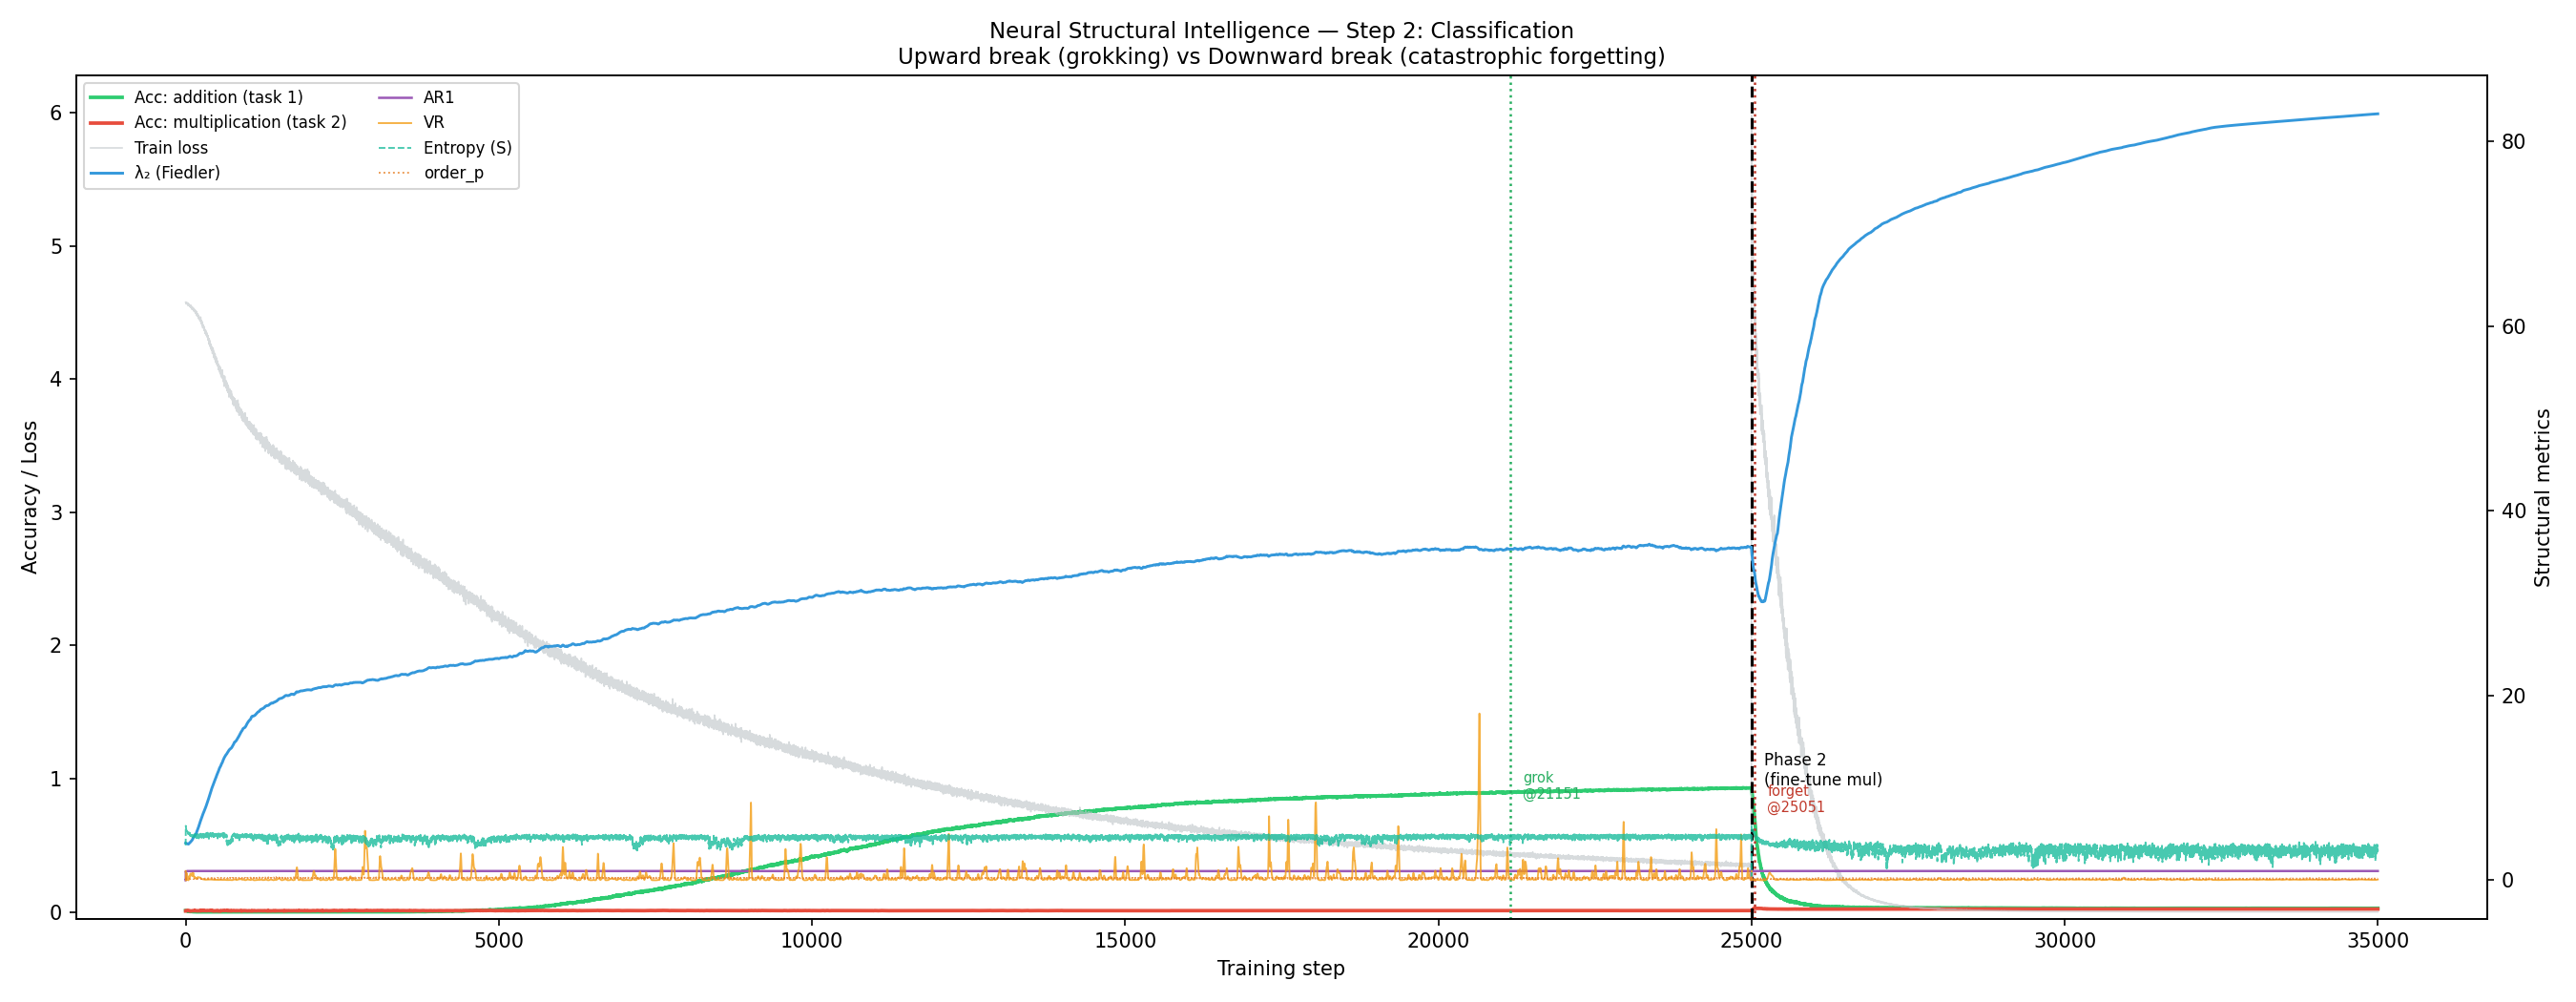
\includegraphics[width=\columnwidth]{results/classification.png}
  \caption{Experiment 2: Classification. Top: $\lambda_2$ trajectory across both phases. The phase transition from grokking (Phase 1) to catastrophic forgetting (Phase 2) is visible as a dip followed by explosive climb — a distinct shape from the monotonic rise of grokking. Bottom: accuracy. The structural signal (dip at step 25,051) precedes accuracy collapse by several hundred steps.}
  \label{fig:classification}
\end{figure}

\subsection{Experiment 3: Steering}

\textbf{Setup}: Phase 1 checkpoint loaded. Two Phase 2 conditions from identical starting weights: unsteered (standard fine-tuning) and steered ($\lambda_2$ slope monitoring with two-stage intervention).

\textbf{Results}: The intervention fired at step 25,013 with addition accuracy still at 87.5\%. $\lambda_2$ slope exceeded the $-0.003$ threshold for 10 consecutive steps, triggering LR reduction and curriculum adjustment. Escalation to fc1 layer freezing occurred when $\lambda_2$ rate exceeded 0.004/step.

\begin{table}[h]
\centering
\caption{Experiment 3: Steering results.}
\label{tab:steering}
\begin{tabular}{lcc}
\toprule
Condition & Addition acc. & $\lambda_2$ (end) \\
\midrule
Unsteered & 2.6\% & 86.46 \\
Steered   & \textbf{91.7\%} & \textbf{35.94} \\
\bottomrule
\end{tabular}
\end{table}

$\lambda_2$ moved by 0.02 in the steered condition versus 50.5 in the unsteered condition, confirming that the structural violence of catastrophic forgetting was contained.

\begin{figure}[h]
  \centering
  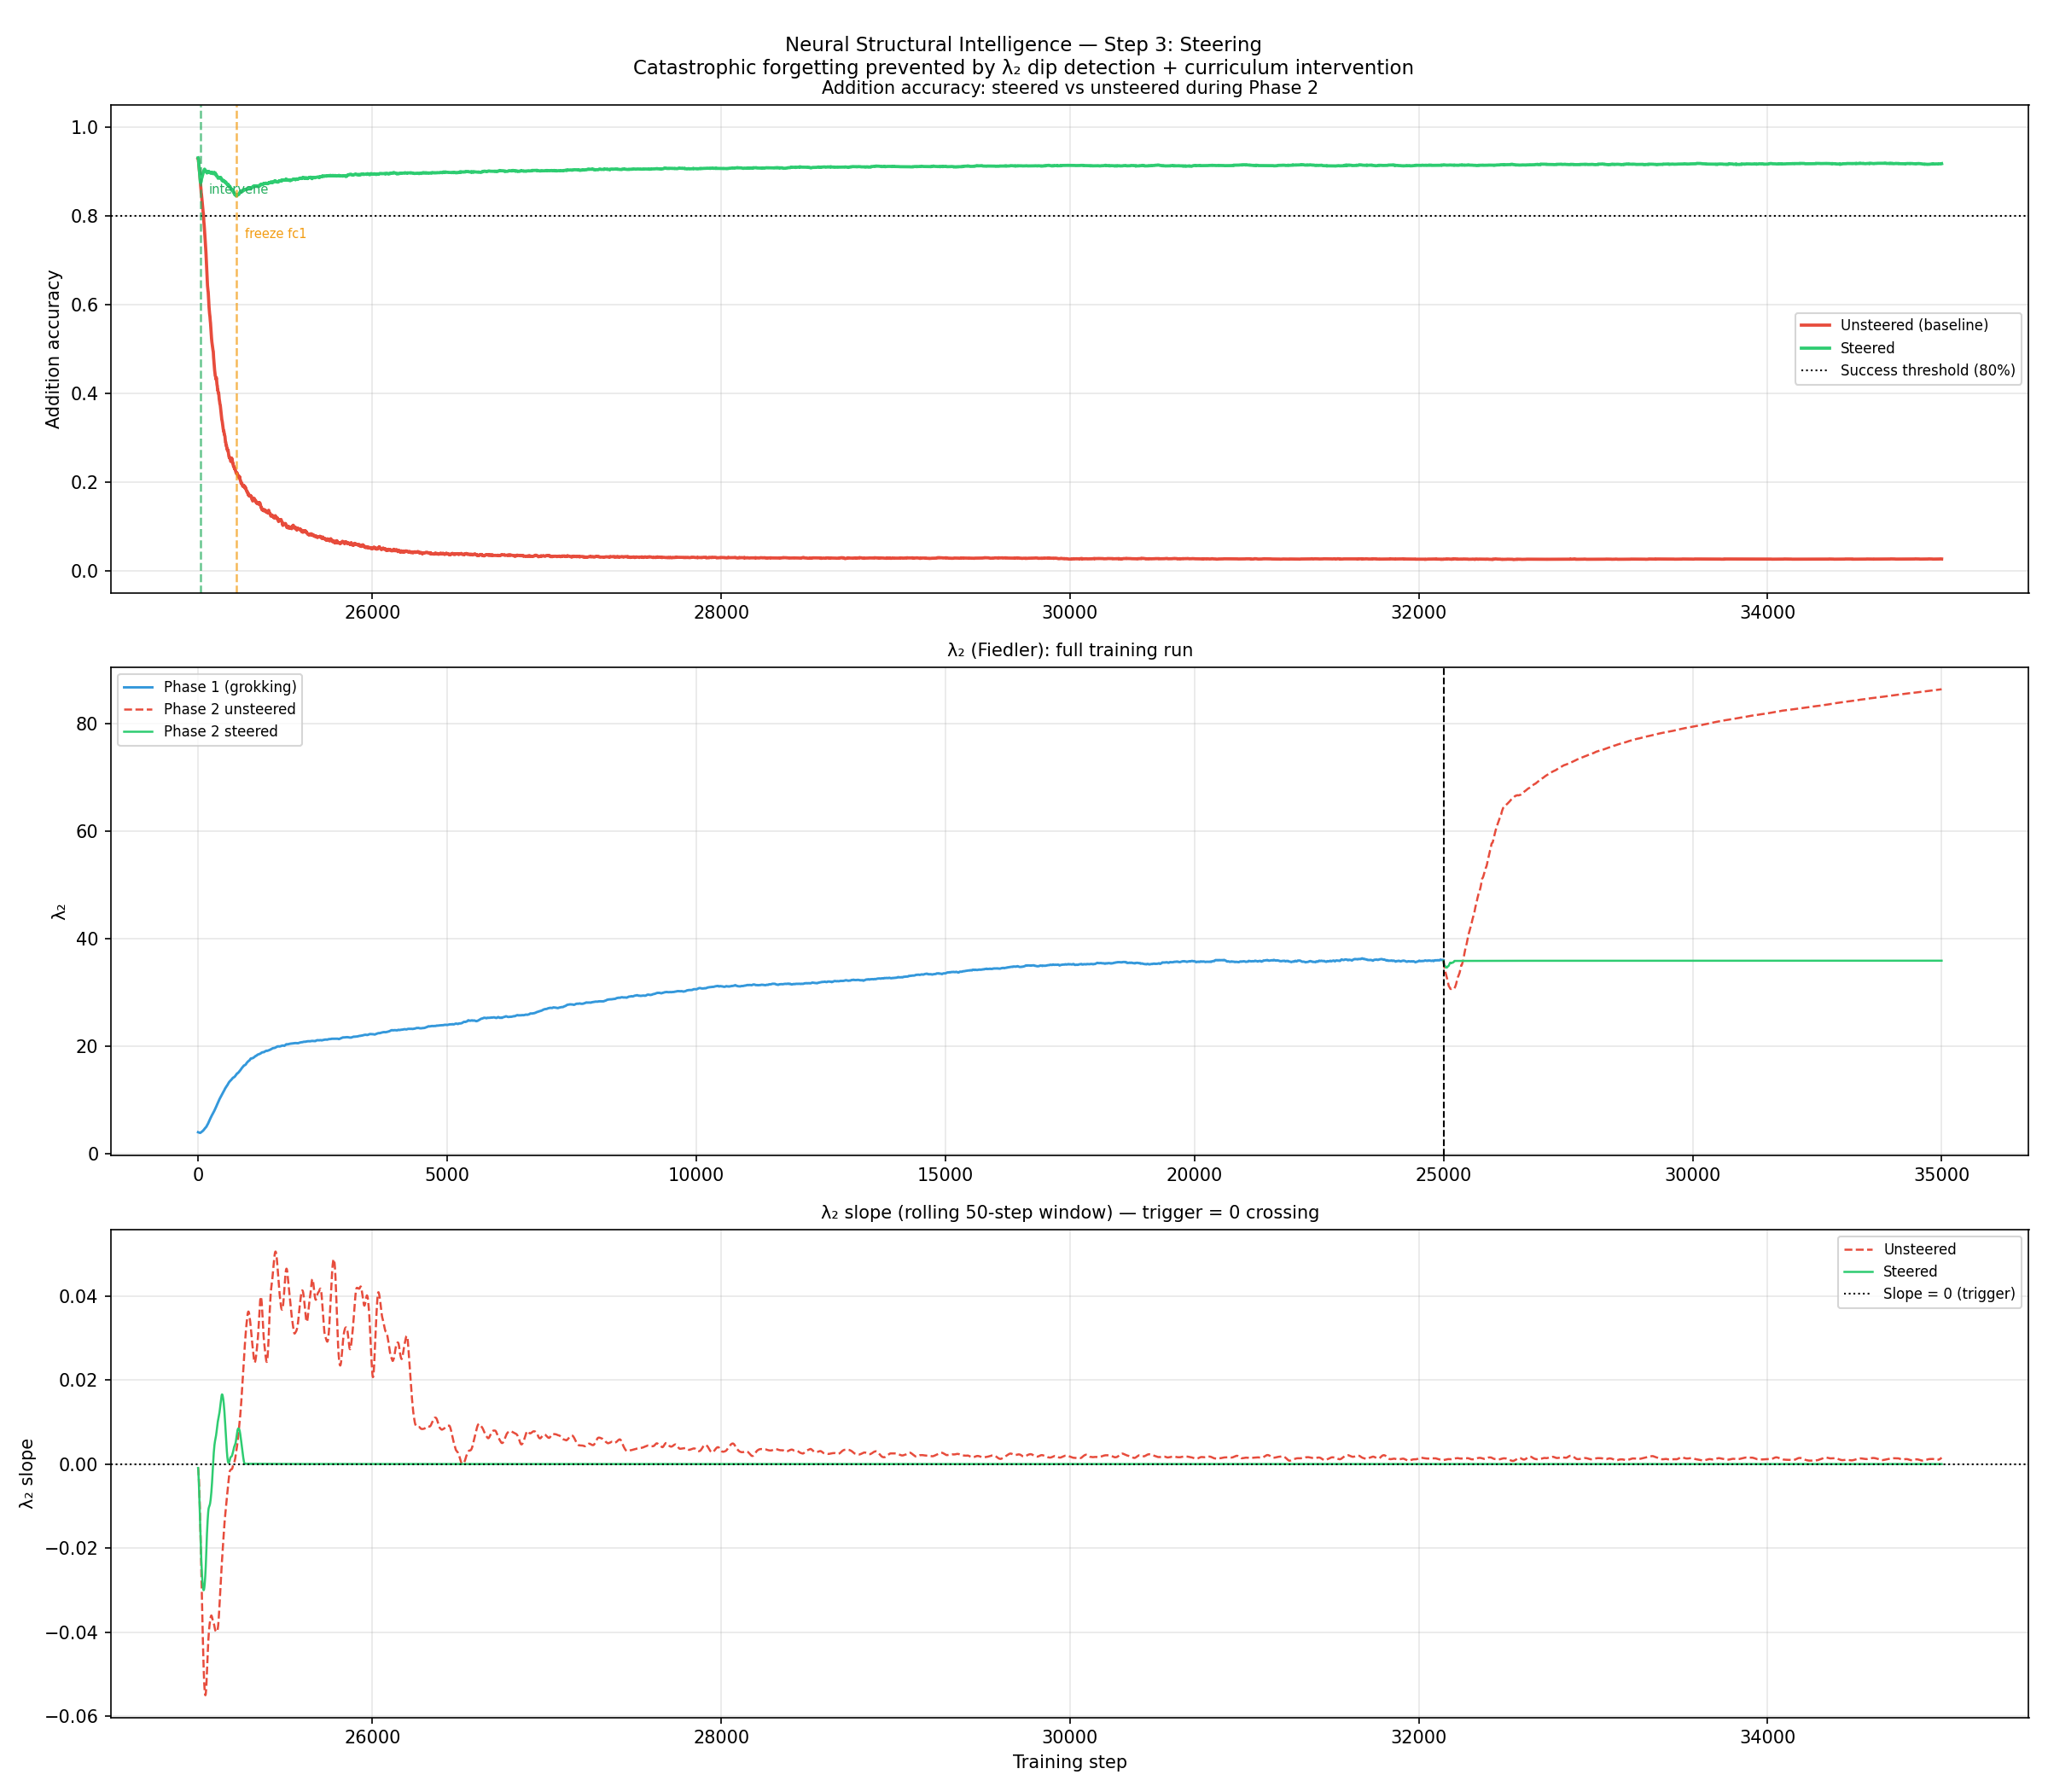
\includegraphics[width=\columnwidth]{results/steering.png}
  \caption{Experiment 3: Steering. $\lambda_2$ trajectory and accuracy for steered versus unsteered conditions. The intervention fires before accuracy collapse (dashed vertical line), holding $\lambda_2$ near its Phase 1 value while the unsteered condition undergoes structural violence.}
  \label{fig:steering}
\end{figure}

\subsection{Experiment 4: Compounding}

\textbf{Setup}: Three sequential tasks (addition mod 97, subtraction mod 97, addition mod 53) with accuracy-anchored controller. Six iterations explored controller designs and architectures.

Iterations v1--v5 on single-head MLPs (128 and 512 units) identified a replay trap: a self-reinforcing loop where accuracy deficits drove replay fractions to 90\%, starving new tasks of gradient bandwidth. All single-head variants converged to approximately equal capacity shares per task ($\approx$25--30\%) regardless of controller configuration. This was diagnosed as output layer competition.

Iteration v6 introduced multi-head architecture: shared representation layer (fc1, 512 units), separate readout head (fc2) per task.

\begin{table}[h]
\centering
\caption{Experiment 4 (v6): Multi-head compounding results.}
\label{tab:compounding}
\begin{tabular}{lcc}
\toprule
Task & Accuracy & Steps to grok \\
\midrule
$(a+b) \bmod 97$ & \textbf{100.0\%} & 4,869 \\
$(a-b) \bmod 97$ & \textbf{100.0\%} & 110 \\
$(a+b) \bmod 53$ & \textbf{97.5\%}  & 101 \\
\bottomrule
\end{tabular}
\end{table}

Controller deficit: 0.000 throughout. Replay: 10\% baseline throughout. The 48$\times$ acceleration from Task A to Task C demonstrates structural priming: each grokking event builds foundations in the shared representation layer that accelerate subsequent tasks.

\begin{figure}[h]
  \centering
  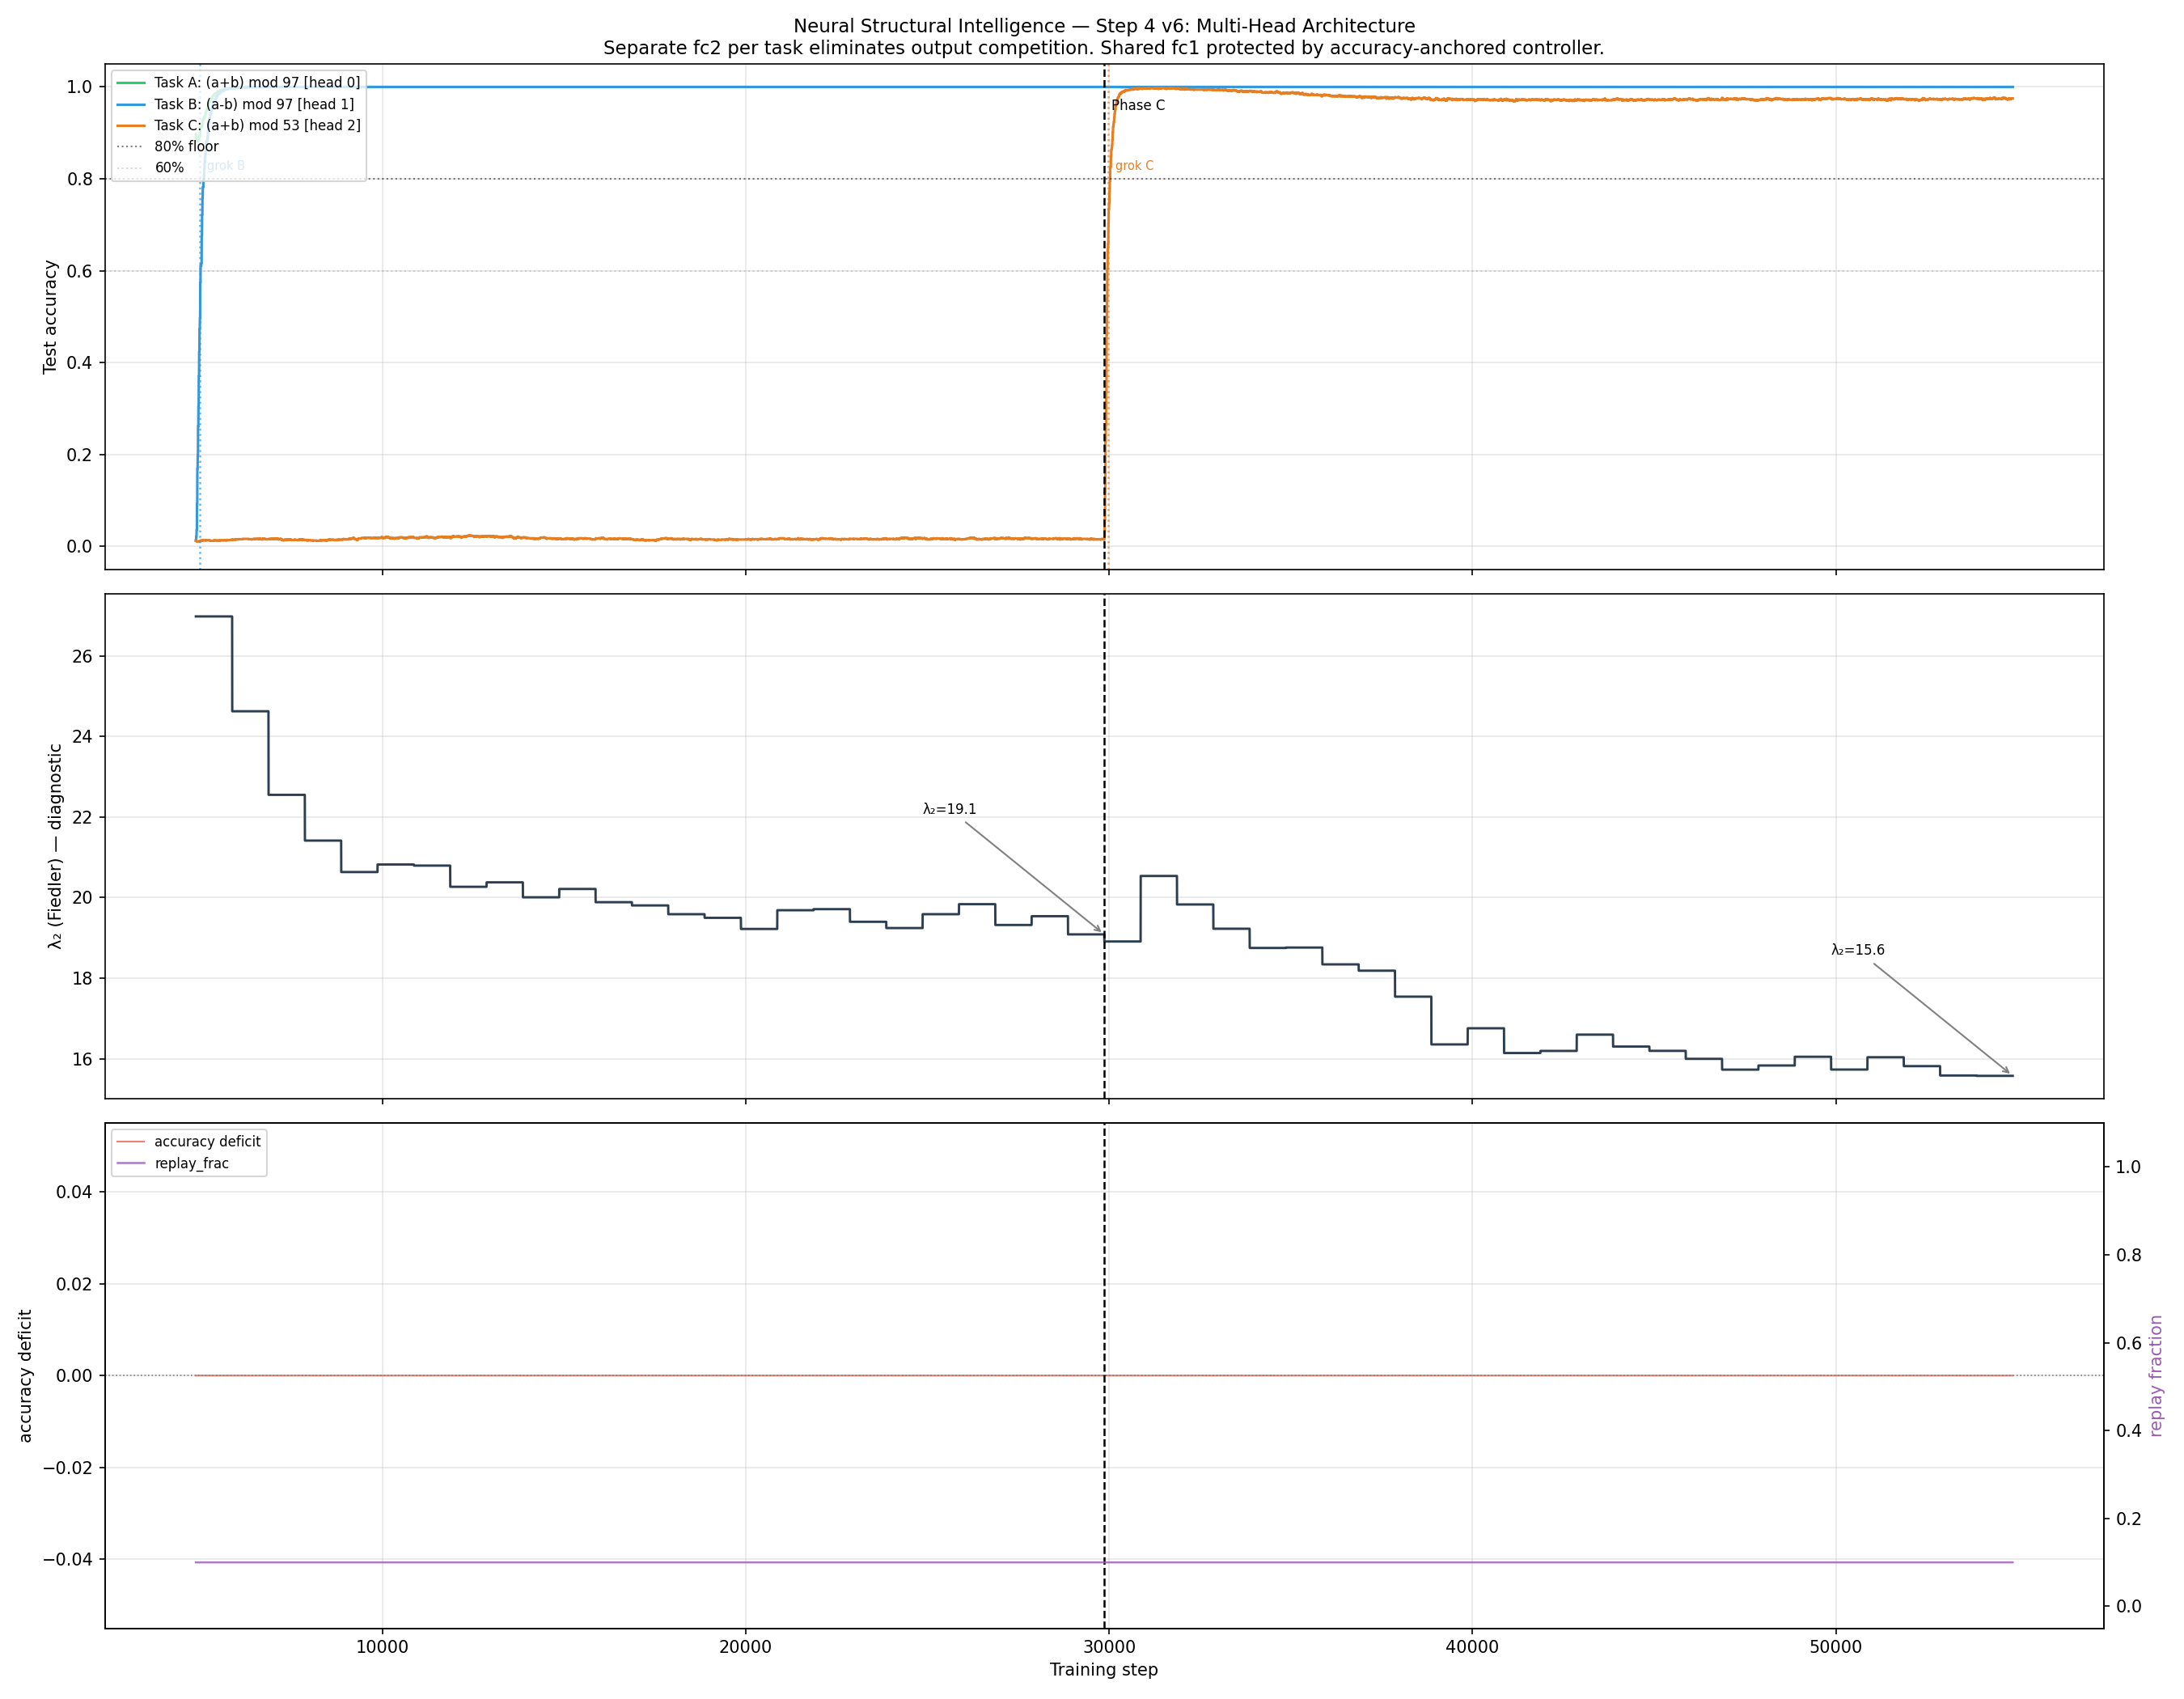
\includegraphics[width=\columnwidth]{results/compounding_v6_multihead.png}
  \caption{Experiment 4 (v6): Multi-head compounding. Accuracy for all three tasks across all phases. Tasks B and C grok in 110 and 101 steps respectively, compared to 4,869 for Task A — structural priming compressing subsequent learning by 48$\times$.}
  \label{fig:compounding}
\end{figure}

\subsection{Experiment 5: Preemptive Curriculum Design}

\textbf{Setup}: 1-layer transformer on three next-token prediction tasks: arithmetic (``$3 + 5 = 8$''), reversed arithmetic (``$8 = 5 + 3$''), and logical syllogisms (``if A then B, A, therefore B''). Task C (logic) introduced after Task A (arithmetic) grokked.

\textbf{Compatibility scoring}: directional gradient conflict weighted by Fiedler sensitivity correctly ranked logic as higher disruption risk than reversed arithmetic. The transformer's attention heads specialise across tasks, producing genuinely differentiated activation subspaces (unlike the MLP where activation overlap was 96\%, making the scoring function undiscriminating).

\begin{table}[h]
\centering
\caption{Experiment 5: Preemptive curriculum results.}
\label{tab:curriculum}
\begin{tabular}{lcc}
\toprule
Condition & Task A acc. & Task C acc. \\
\midrule
Direct (no replay) & 0\% & 82\% \\
Bridged (blend + 10\% replay) & \textbf{100\%} & 83\% \\
\bottomrule
\end{tabular}
\end{table}

The bridging curriculum completely prevented catastrophic forgetting that was total without it.

\textbf{$\lambda_2$ finding}: the bridged condition produced a larger $\lambda_2$ dip than the direct condition. Under hostile takeover, $\lambda_2$ barely moves before the weight graph is overwritten. Under controlled bridging, the topology reorganises gradually, producing a measurable structural signature. Hostile destruction bypasses topology reorganisation; controlled reorganisation is visible in the structural metrics and can be steered.

\begin{figure}[h]
  \centering
  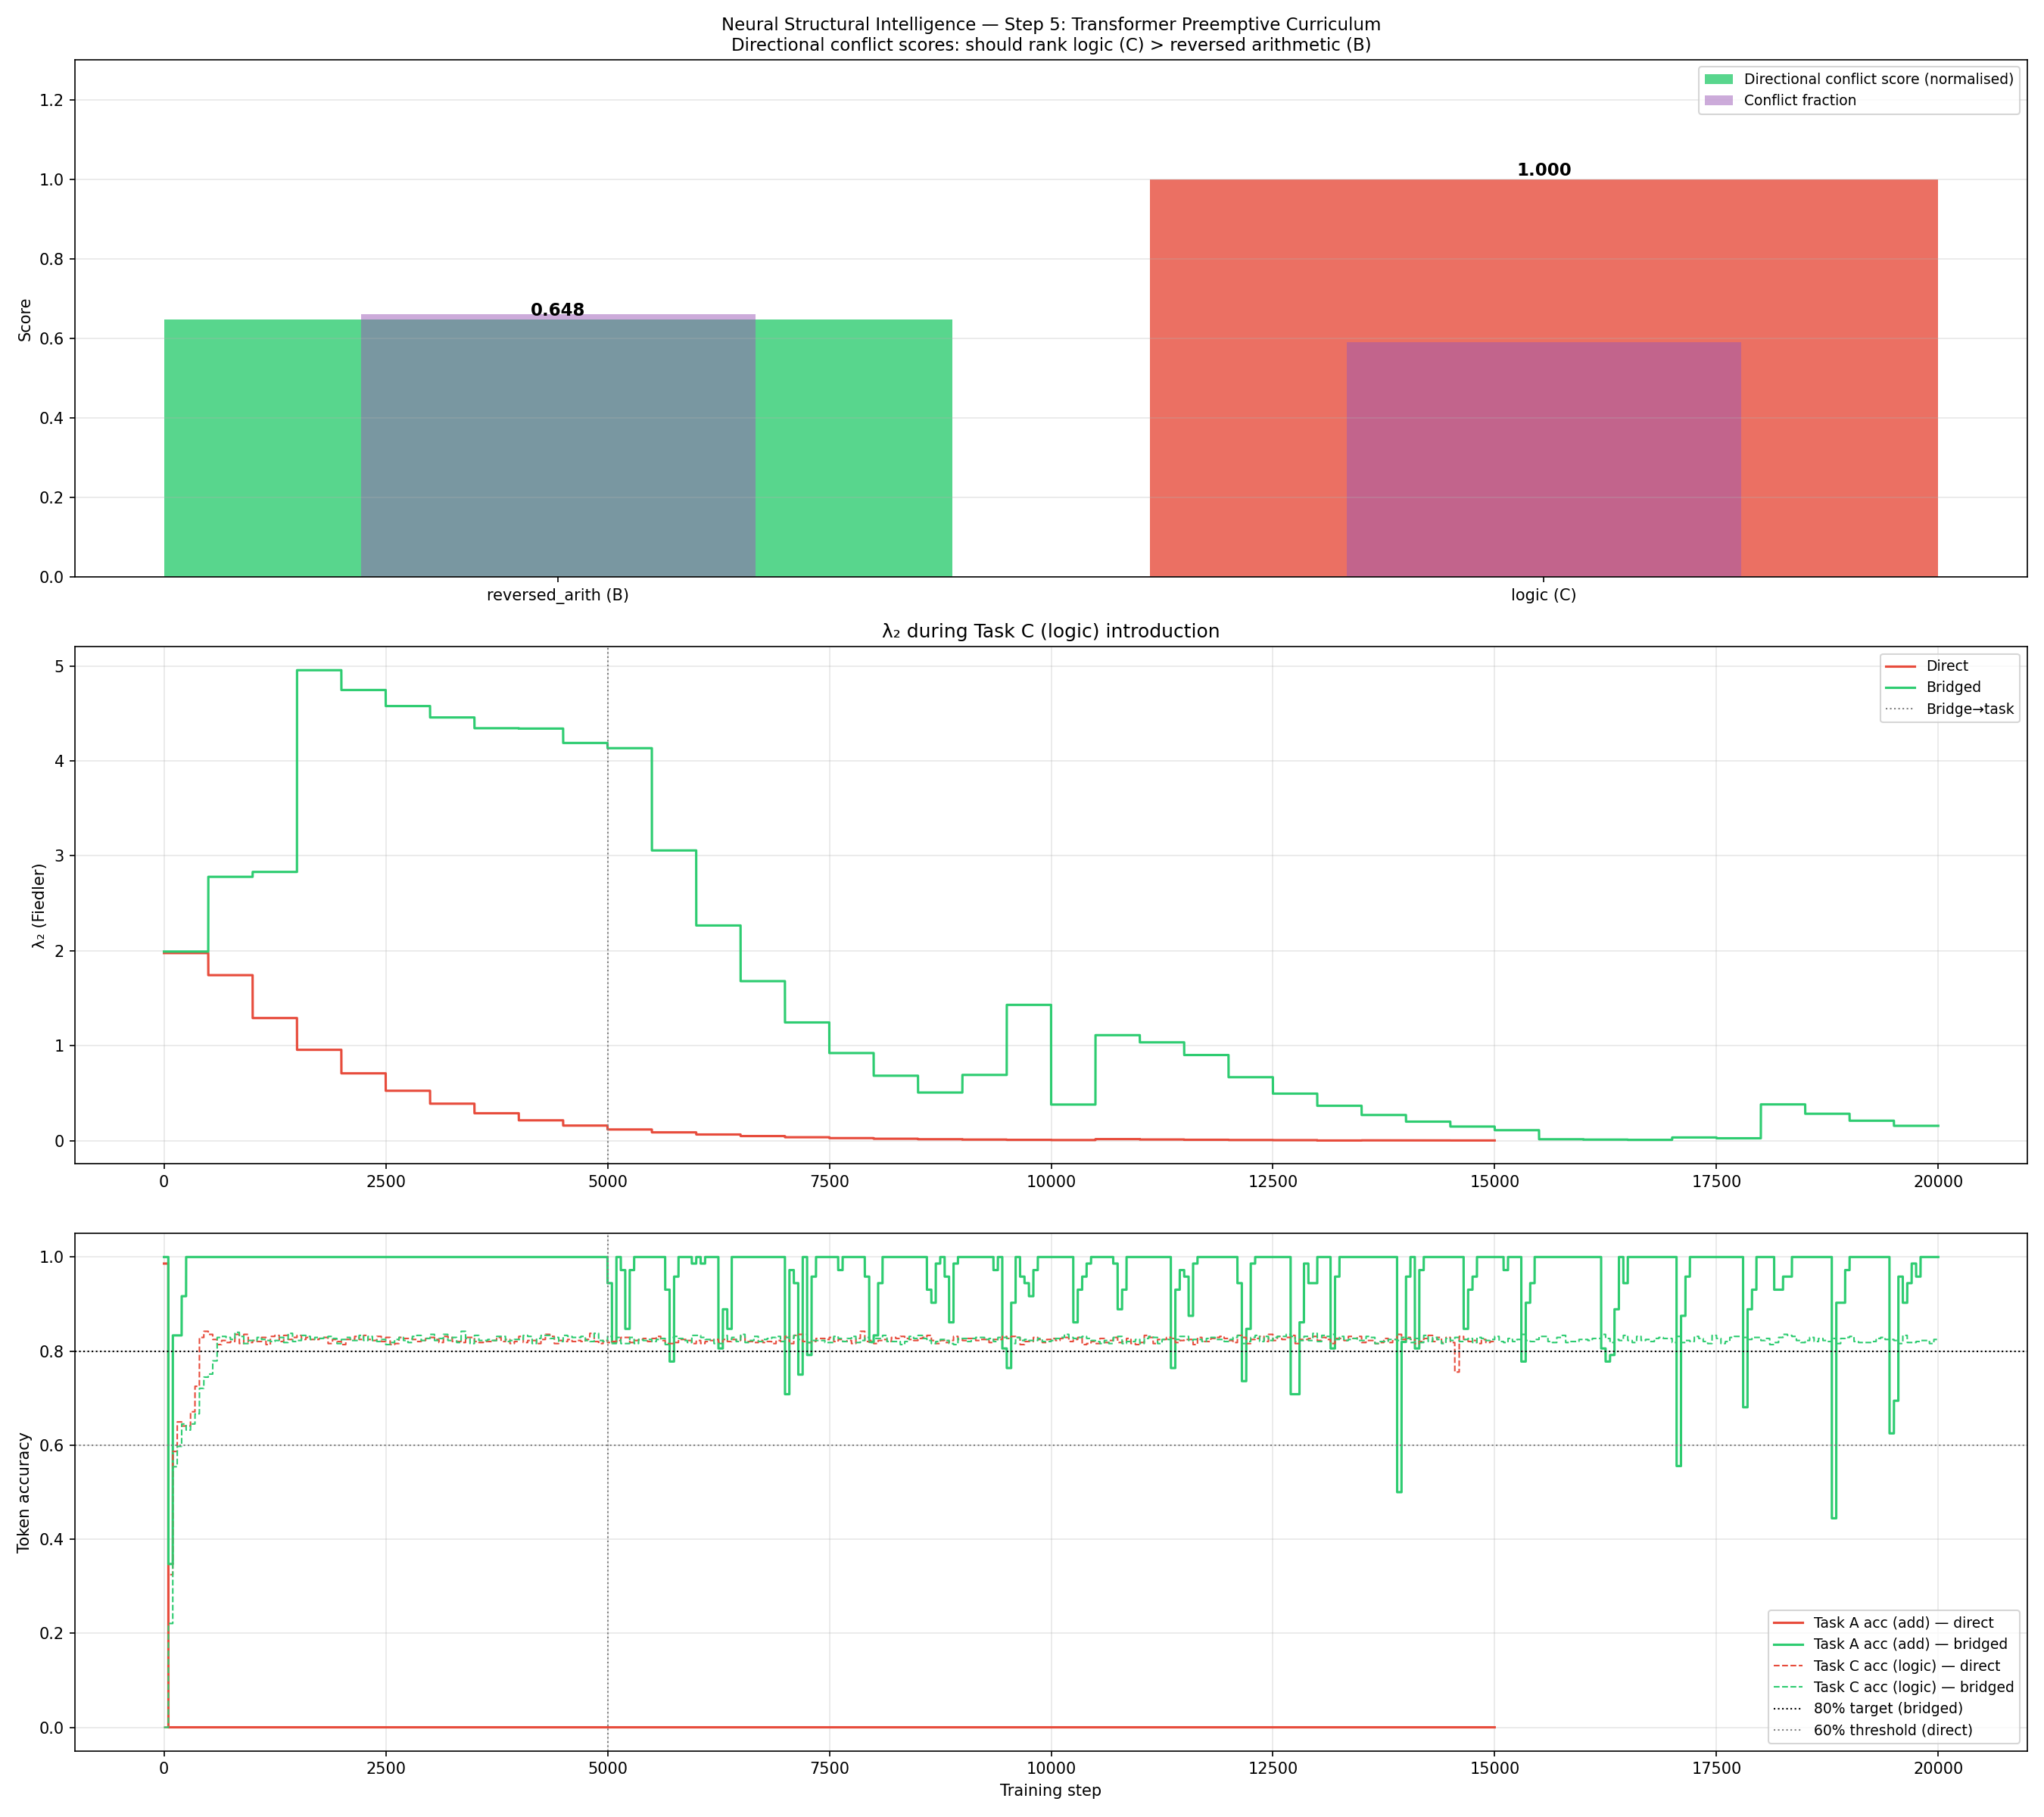
\includegraphics[width=\columnwidth]{results/transformer_step5.png}
  \caption{Experiment 5: Preemptive curriculum on transformer. Top: compatibility scores — logic (C) correctly scored as higher disruption risk than reversed arithmetic (B). Middle: $\lambda_2$ trajectory. Bottom: accuracy for both conditions. Direct introduction causes total forgetting of Task A; bridged introduction preserves it completely.}
  \label{fig:curriculum}
\end{figure}

%% ─────────────────────────────────────────────────────────────────────────────
\section{Discussion}

\subsection{The Structural Correlate of Generalisation}

The $\lambda_2$ trajectory during grokking is a continuous, monotonic correlate of generalisation forming in the weight graph. The network's algebraic connectivity increases steadily for 21,000 steps while the loss function shows nothing. The grok is not a sudden event in the topology — it is the moment that sustained structural preparation manifests in output metrics. This has practical implications: $\lambda_2$ can serve as a training progress indicator that is independent of loss and accuracy.

\subsection{Grokking Versus Forgetting: Shape, Not Direction}

The initial prediction was that $\lambda_2$ would rise for grokking and fall for forgetting. The data revealed a more nuanced signature: both transitions involve rising $\lambda_2$, but at dramatically different rates (0.00128 versus 0.00471/step) and with different shapes (monotonic versus dip-then-explosive-rise). The classification is by shape and rate, not by direction. This is a stronger discriminant than originally hypothesised.

\subsection{The Replay Trap}

The v1--v5 iterations of Experiment 4 characterise a failure mode of proportional replay on capacity-limited single-head networks. The mechanism is precisely identified: accuracy deficit drives replay, which starves new-task gradients, which maintains the deficit. The root cause is architectural (output layer competition), and the resolution is a one-structural-change fix (multi-head readout). The structural monitoring framework correctly diagnosed the problem as architectural rather than dynamic.

\subsection{Structural Priming and Grokking Acceleration}

The 4,869 $\to$ 110 $\to$ 101 step progression across three sequential tasks demonstrates that grokking events build structural foundations that accelerate subsequent learning. The 4.3$\times$ acceleration from 128 to 512 hidden units (21,151 to 4,869 steps on the same task) shows that this priming compounds with capacity.

\subsection{The $\lambda_2$ Surprise in Preemptive Curriculum Design}

Hostile takeover produces a \textit{smaller} $\lambda_2$ dip than controlled bridging. Hostile destruction overwrites the weight graph so rapidly that there is no reorganisation phase. Controlled bridging produces a genuine structural transition that is visible, measurable, and steerable. The most destructive training regimes are structurally invisible — which has implications for training safety: if you cannot see the structural disruption, you cannot prevent it.

\subsection{Limitations}

All experiments use toy tasks (modular arithmetic, simple sequence prediction) on small architectures (128--512 unit MLPs, 40K-parameter transformer). Generalisation to production-scale training is unvalidated. The computational cost of Fiedler value computation scales as $O(n^3)$ for exact methods, requiring approximate methods at scale. The curriculum scoring function was undiscriminating on MLPs due to activation saturation and only worked on the transformer where attention specialisation produced differentiated activation patterns. Scaling behaviour of the structural metrics beyond 512 units is not characterised.

%% ─────────────────────────────────────────────────────────────────────────────
\section{Conclusion}

We have demonstrated that the structural topology of neural network weight graphs, monitored via Fiedler value analysis and Scheffer early warning indicators, provides a predictive signal for phase transitions during training that precedes the loss function by orders of magnitude. The framework detects, classifies, prevents, compounds, and preemptively manages these transitions through five validated experimental steps.

The same mathematical framework applies across architectures (MLP and transformer) and task domains (modular arithmetic and language-like sequence prediction) without modification, consistent with the universality of critical slowing down indicators in complex systems.

The core finding is that shape is signal: the structural topology of the weight graph encodes information about approaching phase transitions that is not available in the loss function. Monitoring this topology in real time enables a class of training interventions that are impossible when the loss function is the only feedback signal.

Future work includes validation at production scale, integration with established continual learning methods, and exploration of the structural priming mechanism as a basis for curriculum-optimised training.

%% ─────────────────────────────────────────────────────────────────────────────
\section*{Reproducibility}

All code, data, and checkpoints are available at \url{https://github.com/EssexRich/neural_si_validation}. Total computation time for all five experiments is under 24 hours on a consumer laptop CPU (Intel i7) with no GPU. The structural monitoring framework requires only PyTorch, NumPy, and SciPy.

%% ─────────────────────────────────────────────────────────────────────────────
\bibliographystyle{plainnat}
\bibliography{references}

\end{document}
